% generated by pramaan render; do not edit
\subsection{Setup}
All results come from a dry run on the quarter ended 30 June 2026, because the September quarter had not been filed when this version was written. The gym covers 245 filings and holds 483 train, 291 dev and 295 test questions; splits are chronological by board meeting date and frozen. Unless stated otherwise, agent results use one fixed random sample of 100 of the 291 dev questions for every configuration, so differences are paired. Only a preregistered sample of 100 of 295 test questions has been read; the other test questions are unread. The guard log records 10 test reads: one per configuration, plus those of a first attempt that a budget-accounting bug invalidated and that was re-run with unchanged settings. The small and strong tiers are \texttt{claude-haiku-4-5} and \texttt{claude-sonnet-5-5}. \emph{Verified accuracy} counts an answer only if it is correct and its citations check out. Confidence intervals are 95\% bootstrap intervals clustered by filing; paired differences use the same clustered bootstrap and McNemar's test.

\subsection{E1: is the gym valid?}
When the rules reader found the printed row, the PDF and the XBRL agreed on 88.5\% of 2593 facts. A further 1874 facts had no matching row and 606 no unit header, so they say nothing about agreement. 62 facts were dropped because the XBRL element and the printed row are defined differently (for example consolidated profit before tax with and without the share of associates). Gold evidence was located for 89.6\% of 719 facts on digital pages, 77.9\% of 4354 on pages with an embedded OCR layer, and almost never (2.9\%) for the 38 filings where no results page was detected; those filings contribute no questions. Human validation of the 100-question sample has not been done.

\subsection{E2: what does each retrieval stage buy?}
Dense retrieval alone beats BM25 by a wide margin on numeric table pages, and fusing the two with reciprocal rank fusion is \emph{worse} than dense alone on nDCG@10 (0.829 against 0.911). Row documents, which render each table row as a retrievable unit, lift nDCG@10 to 0.939. The off-the-shelf cross-encoder then \emph{lowers} it to 0.745, because it cannot tell near identical statement pages apart. Fine-tuned on 2922 train-split pairs whose labels come from XBRL for free, it reaches 0.987 (recall@1 0.488 to 0.976). The fine-tuning pairs and their negatives come from train filings only; an earlier version drew negatives from dev and test pages and was discarded and retrained, which changed nDCG@10 by less than 0.002. Queries are synthetic template questions from one quarter, so this measures generalisation to new companies and filings, not to free-form analyst wording.
\begin{table}[H]\centering\small\begin{tabular}{lrrr}\toprule
stages (company-filtered) & R@1 & R@5 & nDCG@10 \\\midrule
R1 BM25 only & 0.440 & 0.860 & 0.694 \\
R1 dense only & 0.797 & 0.990 & 0.911 \\
R1+R2 BM25+dense RRF & 0.633 & 0.986 & 0.829 \\
R1+R2 with row docs & 0.855 & 1.000 & 0.939 \\
R1-R3 + off-the-shelf cross-encoder & 0.488 & 0.918 & 0.745 \\
R1-R3 + fine-tuned cross-encoder & 0.976 & 0.990 & 0.987 \\
\bottomrule\end{tabular}\caption{Retrieval stages on 207 dev queries.}\end{table}

\subsection{E3: the agent against baselines}
\begin{table}[H]\centering\small\begin{tabular}{lrrrrrr}\toprule
config & n & verified acc. (CI) & abstain & \$/question & \$/verified correct & p50 s \\\midrule
\texttt{B0\_naive\_rag} & 100 & 10.0 (5--16) & 87 & 0.0025 & 0.0253 & 0.1 \\
\texttt{small\_only} & 100 & 71.0 (61--80) & 33 & 0.0146 & 0.0205 & 19.1 \\
\texttt{strong\_only} & 100 & 80.0 (68--90) & 26 & 0.0305 & 0.0381 & 14.9 \\
\texttt{cascade} & 100 & 71.0 (61--80) & 33 & 0.0180 & 0.0254 & 15.3 \\
\bottomrule\end{tabular}\caption{Specified configurations on the same dev sample. Costs are real API spend recorded at the original price of cached calls; latency is wall clock plus the recorded latency of cached calls.}\label{tab:main}\end{table}
The agent beats the naive RAG baseline by +61.0 points (95\% CI +50.0 to +70.1; 62 fixed, 1 broken; McNemar $p < 0.001$). Naive RAG is cheap per question but almost always wrong or silent, so per verified correct answer the small-model agent is cheaper (\$0.0205 against \$0.0253). The long-context baseline B1 was not run: it sends whole PDFs, and the cost estimator puts it far above the budget of this study, so the second half of H3 is untested. The strong model gains +9.0 points (95\% CI -2.9 to +20.5; 16 fixed, 7 broken; McNemar $p = 0.093$) over the small one, a difference that does not reach significance at this sample size. \textbf{H1 is not supported as preregistered.} The specified cascade differs from \texttt{strong\_only} by -9.0 points (95\% CI -20.5 to +2.9; 7 fixed, 16 broken; McNemar $p = 0.093$), so the preregistered condition (within two points of \texttt{strong\_only} and cheaper) fails on accuracy, and it is dominated by \texttt{small\_only} (it gave identical verified answers on every question, at a higher cost per question). Reflection ran on the questions that hard-failed verification but ended in ``value not found'' abstentions, and escalation fires only on a hard failure after reflection, so the strong model was consulted on almost no questions.
\paragraph{Offline baseline.} A deterministic rules reader with no language model (clearly labelled offline, on all 291 dev questions) reaches 50.5\% with the off-the-shelf reranker and 60.1\% with the fine-tuned one. It is precise but silent: it abstains on about half of the answerable questions.
\begin{figure}[H]\centering\IfFileExists{../results/figures/fig1_pareto.png}{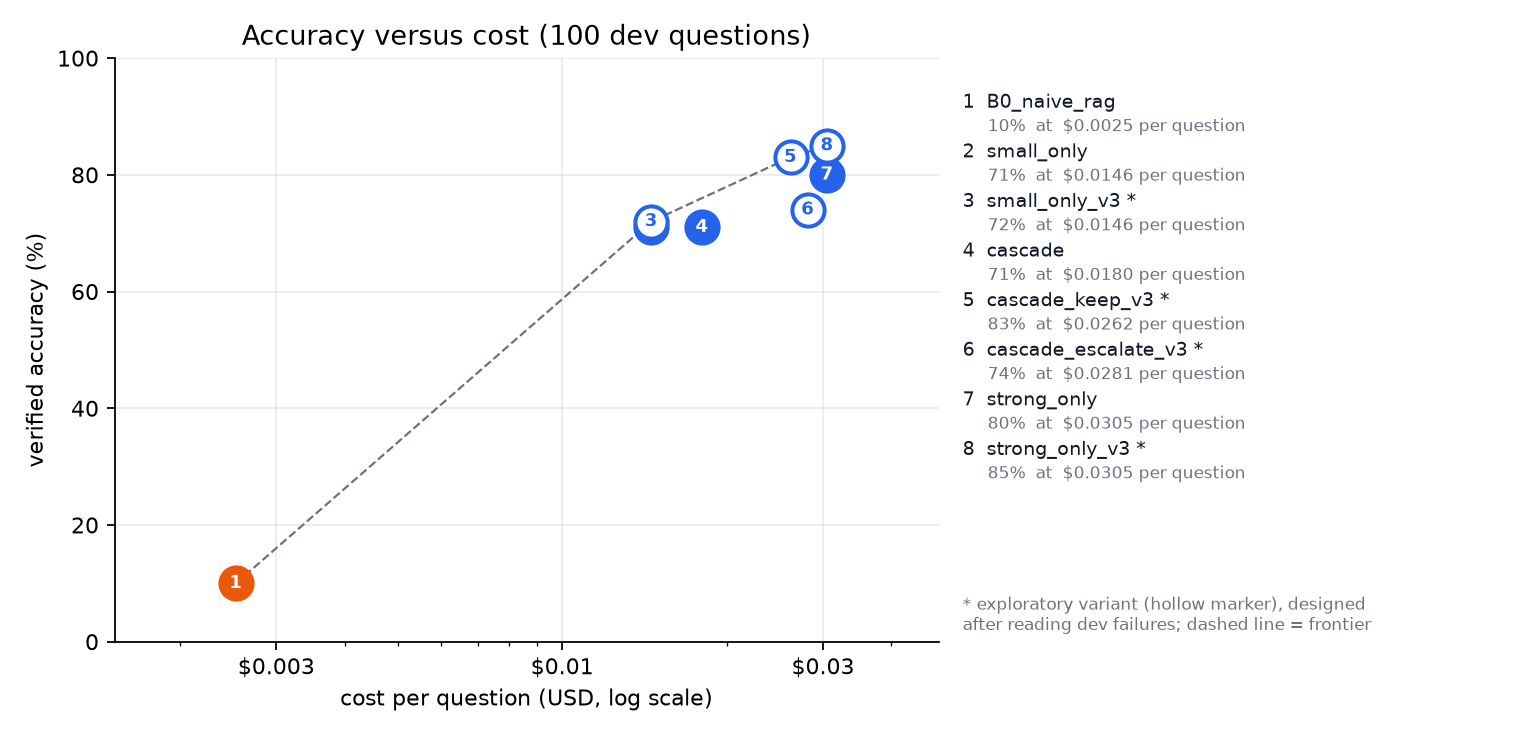
\includegraphics[width=\linewidth]{../results/figures/fig1_pareto.png}}{}
\caption{Verified accuracy against cost per question. Hollow markers are exploratory variants.}\label{fig:pareto}\end{figure}

\subsection{Exploratory: why the cascade did not help}
\emph{The variants in this subsection were designed after reading failures on the dev sample, so their numbers are optimistic and are marked $^{*}$; they need confirming on questions not used to design them, and the specified configurations stay in every table.}

\paragraph{The verifier discards correct answers.} Grading the stored drafts of abstained answerable questions shows that \texttt{strong\_only} threw away 6 correct answers (V3 5, V4 1) and \texttt{small\_only} 4 (V2 2, V3 1, V4 1); 12 and 4 further questions ended with no numeric draft at all because the model itself reported the value as not found. All 6 V3 (unit sanity) false rejects have one shape: a percent answer computed from two inputs cited on a single page. There the page's unit header cancels, so a missing header cannot hide a scale error. Relaxing V3 for exactly that case (inputs on different pages and absolute values keep the strict rule) is the variant \texttt{small\_only\_v3} / \texttt{strong\_only\_v3}. It recovers +5.0 points (95\% CI +0.0 to +11.2; 5 fixed, 0 broken; McNemar $p = 0.062$) for the strong model and +1.0 points (95\% CI +0.0 to +3.3; 1 fixed, 0 broken; McNemar $p = 1.000$) for the small one, and the number of wrong answers did not change (2 to 2 and 4 to 4), so it added no false accepts in this sample.

\paragraph{Escalation was broken by a page ban.} Letting the cascade escalate when the small model gives up (\texttt{cascade\_escalate\_v3}) escalated 24 questions, yet the strong tier inside the cascade answered only 2 of them correctly while standalone \texttt{strong\_only\_v3} answers 16 of the same 24. The cause is that after a failed verification the graph bans every page that produced a value, so a retry or an escalation cannot use the right page when the failure was a verifier false reject or a reading slip on it. Keeping failed pages available (\texttt{cascade\_keep\_v3}), the only change, adds +9.0 points (95\% CI +3.1 to +16.7; 9 fixed, 0 broken; McNemar $p = 0.004$). Against \texttt{strong\_only\_v3} the repaired cascade differs by -2.0 points (95\% CI -8.8 to +4.9; 4 fixed, 6 broken; McNemar $p = 0.754$) at lower cost per question, which is too imprecise to settle the two-point margin of H1. Even so, inside the cascade the strong tier answered 9 of 22 escalated questions against 14 standalone, so a gap remains.
\begin{table}[H]\centering\small\begin{tabular}{lrrrrrr}\toprule
config & n & verified acc. (CI) & abstain & \$/question & \$/verified correct & p50 s \\\midrule
\texttt{small\_only\_v3}$^{*}$ & 100 & 72.0 (62--81) & 32 & 0.0146 & 0.0202 & 19.5 \\
\texttt{strong\_only\_v3}$^{*}$ & 100 & 85.0 (77--92) & 21 & 0.0305 & 0.0359 & 13.8 \\
\texttt{cascade\_escalate\_v3}$^{*}$ & 100 & 74.0 (65--83) & 27 & 0.0281 & 0.0380 & 16.5 \\
\texttt{cascade\_keep\_v3}$^{*}$ & 100 & 83.0 (74--90) & 21 & 0.0262 & 0.0315 & 20.0 \\
\bottomrule\end{tabular}\caption{Exploratory variants ($^{*}$: designed after reading dev failures).}\label{tab:expl}\end{table}

\subsection{Held-out test sample}
Following Addendum A of the preregistration (written after the dev results and before any test access), every configuration ran on the same seeded random sample of test questions. Only a preregistered sample of 100 of 295 test questions has been read; the other test questions are unread. The guard log records 10 test reads: one per configuration, plus those of a first attempt that a budget-accounting bug invalidated and that was re-run with unchanged settings. Decision rules were fixed in advance and are applied mechanically below. 
\begin{table}[H]\centering\small\begin{tabular}{lrrrrrr}\toprule
config & n & verified acc. (CI) & abstain & \$/question & \$/verified correct & p50 s \\\midrule
\texttt{B0\_naive\_rag} & 100 & 9.0 (4--15) & 92 & 0.0025 & 0.0282 & 2.5 \\
\texttt{small\_only} & 100 & 58.0 (46--70) & 43 & 0.0131 & 0.0225 & 16.8 \\
\texttt{strong\_only} & 100 & 70.0 (59--81) & 29 & 0.0273 & 0.0390 & 13.9 \\
\texttt{cascade} & 100 & 58.0 (46--70) & 43 & 0.0160 & 0.0275 & 16.3 \\
\texttt{small\_only\_v3}$^{*}$ & 100 & 59.0 (47--71) & 42 & 0.0131 & 0.0221 & 16.8 \\
\texttt{strong\_only\_v3}$^{*}$ & 100 & 73.0 (61--84) & 26 & 0.0273 & 0.0374 & 17.0 \\
\texttt{cascade\_keep\_v3}$^{*}$ & 100 & 70.0 (57--83) & 26 & 0.0265 & 0.0379 & 17.5 \\
\bottomrule\end{tabular}\caption{Held-out test sample ($^{*}$: exploratory variants, designed on dev).}\label{tab:test}\end{table}
\paragraph{H3, first half.} The small-model agent beats naive RAG by +49.0 points (95\% CI +36.6 to +61.1; 50 fixed, 1 broken; McNemar $p < 0.001$).
\paragraph{H1 as preregistered: not supported.} \texttt{cascade} minus \texttt{strong\_only} is -12.0 points (95\% CI -21.4 to -3.0; 5 fixed, 17 broken; McNemar $p = 0.017$); cost per question \$0.0160 against \$0.0273. The rule requires the lower end of the interval to be at least $-2$ points and the cascade to be cheaper.
\paragraph{Exploratory variants.} \texttt{small\_only\_v3} minus \texttt{small\_only}: +1.0 points (95\% CI +0.0 to +3.4; 1 fixed, 0 broken; McNemar $p = 1.000$), not confirmed (rule: lower end of the interval above zero); \texttt{strong\_only\_v3} minus \texttt{strong\_only}: +3.0 points (95\% CI +0.0 to +7.0; 3 fixed, 0 broken; McNemar $p = 0.250$), not confirmed (rule: lower end of the interval above zero); \texttt{cascade\_keep\_v3} minus \texttt{cascade}: +12.0 points (95\% CI +5.6 to +19.4; 12 fixed, 0 broken; McNemar $p < 0.001$), confirmed (rule: lower end of the interval above zero). 1 of 3 evaluated variants is confirmed; a confirmed variant is promoted to the headline only after the full test run, and the others stay exploratory.
\paragraph{Cost and accuracy of the repaired cascade.} \texttt{cascade\_keep\_v3} minus \texttt{strong\_only\_v3} is -3.0 points (95\% CI -10.0 to +3.8; 5 fixed, 8 broken; McNemar $p = 0.581$), at \$0.0265 against \$0.0273 per question.
\paragraph{Dev to test.} Verified accuracy, \texttt{B0\_naive\_rag} 10.0\% on dev and 9.0\% on test; \texttt{small\_only} 71.0\% on dev and 58.0\% on test; \texttt{strong\_only} 80.0\% on dev and 70.0\% on test; \texttt{cascade} 71.0\% on dev and 58.0\% on test. Splits are chronological, so the test filings are the later ones in the quarter; the shift is reported, not corrected.

\subsection{E4: does it know when it does not know?}
On the live episodes of \texttt{cascade\_keep\_v3} (exploratory, n=100) the base accuracy is 83.0\%; abstaining on the least confident 10\% lifts selective accuracy to 92.2\%, and at the threshold chosen for a 95\% target the agent answers 87.0\% of questions with 95.4\% accuracy (threshold chosen on the same episodes, so in sample). A logistic calibrator over verifier results, retrieval margin and retries has a cross-validated expected calibration error of 0.084, but it does \emph{not} beat the model's own stated confidence: AURC 0.097 calibrated against 0.047 raw (lower is better). Figure~\ref{fig:rc} shows both curves.
\begin{figure}[H]\centering\IfFileExists{../results/figures/fig2_risk_coverage.png}{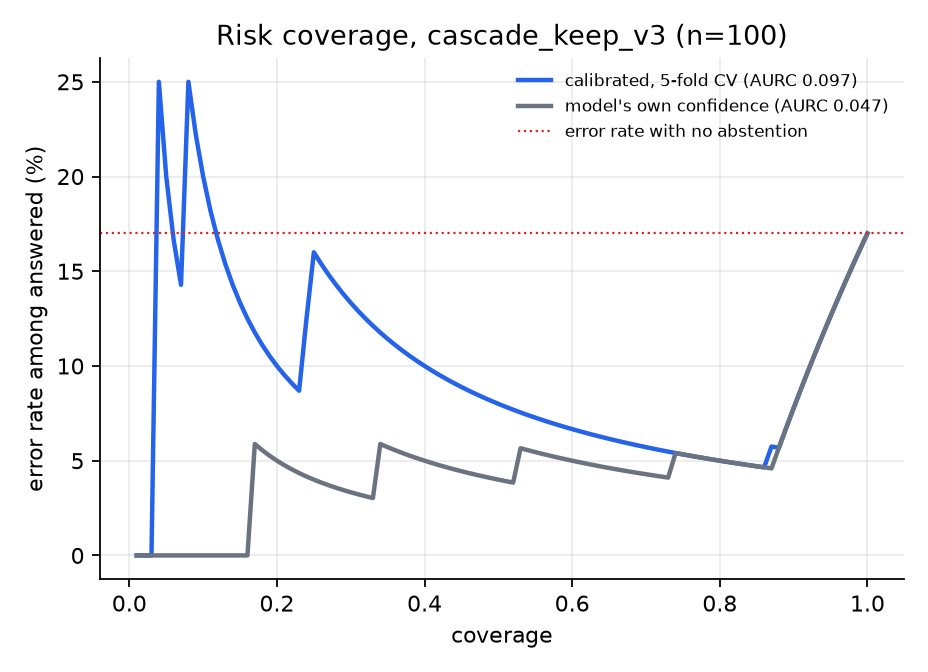
\includegraphics[width=.62\linewidth]{../results/figures/fig2_risk_coverage.png}}{}
\caption{Risk-coverage curves.}\label{fig:rc}\end{figure}

\subsection{E6: where does it fail?}
Attribution was run on the offline rules agent only (117 failures; the live agent has not been attributed because counterfactual replay costs API calls). Failures by stage: intent 33, retrieval 2, rerank 3, read 42, plan or compute 3, citation 1, verifier 33. Retrieval and rerank together explain 4\%, so once the reranker is fine-tuned retrieval is no longer the bottleneck. Injecting the gold table values flips 18\% of failures, the gold page at rank one 3\%, and the gold intent 0\%; most failures are abstentions on answerable questions, which none of these injections addresses. The intent stage is probably a non-causal label (stages are assigned earliest first), and the live agent's stage distribution will differ.

\subsection{E8: what does the season show?}
Over 245 filings the XBRL arrived a median 72 minutes after the results PDF (quartiles 25 and 164, 95th percentile 317); the PDF came first for 95.1\% of filings, and 21.2\% of XBRL files arrived more than three hours later. 6.1\% of filings had at least one revised XBRL, which the gold handling must follow. This lag is what the self-grading loop uses: answer when the PDF lands, grade when the XBRL arrives.
